\section{Consequences for alternatives and ownership}\label{sec:consequences}
The frontier distinguishes more charging flexibility from a physically
implementable hull optimum. Figure~\ref{fig:frontier} illustrates the
two-service specialization in Appendix~\ref{sec:construction}. Two services
each use 15 kWh; a 20 kWh bus can cover both only by buying 10 kWh between
them. Two buses can instead vary early purchases continuously from 0 to 10,
but incur an additional vehicle fee. Under the stated full-refill resources,
fee 7 and quadratic supply function, the physical value is 97 and the hull
value is 94.8875. The energy projection is an interval in both cases; its
operating-cost labels make the difference.

\begin{figure}[t]
\centering
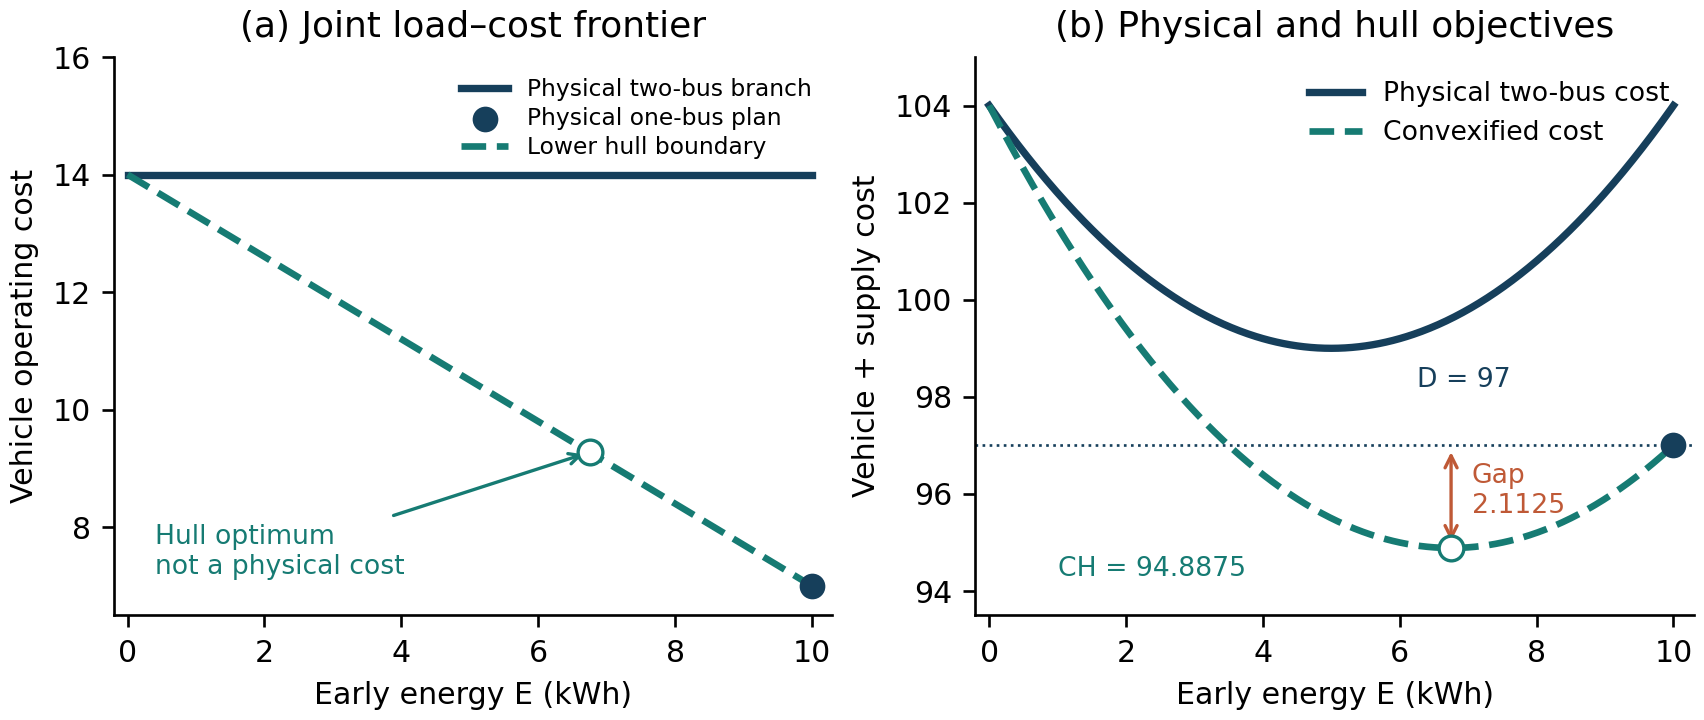
\includegraphics[width=\textwidth]{figures-v3/physical_cost_frontier.png}
\caption{The two-service specialization of Appendix~\ref{sec:construction}.
Every early load from 0 to 10 is feasible with two buses, but the lower
interpolated operating cost is not a physical fleet cost at an interior
load. Adding convex supply cost makes this distinction consequential.
The curves illustrate proved formulas, not sampled experimental data.}
\label{fig:frontier}
\end{figure}

Adding alternatives cannot reduce a retained plan's regret at its unchanged
own price: the minimum competing bill can only decrease. Nevertheless, a
new plan can restore support by implementing a new hull optimum. The exact
equipment analysis in Appendix~\ref{sec:expansion} shows both outcomes.
For the stated nominal example, energy-consuming movement additions under
unchanged charging access and equipment preserve both planning values.
A battery 25 bus at fee 7 instead attains $D=\CH=92$. Raising its fee to 8
gives $D=93$ but $\CH=92.95$: being cheaper than the \emph{old} hull value
does not settle the enlarged problem. These claims retain the original
services, full inventory accounting and the explicit resource assumptions;
they are not universal statements about new routes or battery investments.

Ownership changes the deviation being priced. Appendix~\ref{sec:ownership}
gives a physically realizable replication with all crossmatchings retained,
charging resources proportional to fleet size and supply curvature
proportional to $1/n$. Its planning gap tends to zero, yet along a specified
subsequence one whole owner's absolute own-price regret tends to $351/40$.
For separately owned service pairs with \emph{reserved} charging rights,
individual regret instead vanishes; per-bus and relative whole-owner regret
also vanish. No unilateral-equilibrium claim is made for unreserved shared
chargers or an operator anticipating a tariff reset.

The uniform controls matter. For a compact physical load set of diameter
$R_K$, a differentiable $\mu$-strongly convex supply function with
$\Lambda$-Lipschitz gradient gives the classical explanatory bound
\[
 \Delta\le r(x;\nabla F(u(x)))\le
 \Delta+\Lambda R_K\sqrt{2\Delta/\mu}
\]
at each physical planner optimum, in one fixed load-space norm
(Proposition~\ref{prop:regretbound}). Thus uniformly bounded diameter and
smoothness, and uniformly positive curvature, make that regret vanish with
the planning gap. The replication changes these constants with $n$, so it
does not contradict this conclusion. The bound is convex-analysis
interpretation, not a new general price-support or learning theorem.
